\documentclass[a4paper]{article}

\usepackage[margin=2.5cm]{geometry}
\usepackage[pdftex]{graphicx}
\usepackage[utf8]{inputenc}
\usepackage[T1]{fontenc}
\usepackage{textcomp}
\usepackage{babel}
\usepackage{amsmath, amssymb}
\usepackage[colorlinks=true,linkcolor=blue]{hyperref}
\usepackage{float}
\usepackage{mathrsfs}
%\usepackage{enumitem}
%% for identity function 1:
\usepackage{bbm}
%%For category theory diagrams:
%\usepackage{tikz-cd}
%%For code (e.g. python) in latex:
%\usepackage{listings}
%
%Usage: 
%\begin{lstlisting}[language=Python]
%\end{lstlisting}

\newcommand{\incfig}[2][1]{%
\def\svgwidth{#1\columnwidth}
\import{./figures/}{#2.pdf_tex}
}


% figure support
\usepackage{import}
\usepackage{xifthen}
\pdfminorversion=7
\usepackage{pdfpages}
\usepackage{transparent}

\pdfsuppresswarningpagegroup=1

\setlength\parindent{0pt}

\newcommand{\qed}{\tag*{$\blacksquare$}}
\newcommand{\qedwhite}{\hfill \ensuremath{\Box}}

%Inequalities
\newcommand{\cycsum}{\sum_{\mathrm{cyc}}}
\newcommand{\symsum}{\sum_{\mathrm{sym}}}
\newcommand{\cycprod}{\prod_{\mathrm{cyc}}}
\newcommand{\symprod}{\prod_{\mathrm{sym}}}

%Linear Algebra

\DeclareMathOperator{\Span}{span}
\DeclareMathOperator{\Ima}{Im}
\DeclareMathOperator{\diag}{diag}
\DeclareMathOperator{\Ker}{Ker}
\DeclareMathOperator{\ob}{ob}
\DeclareMathOperator{\Hom}{Hom}
\DeclareMathOperator{\sk}{sk}
\DeclareMathOperator{\Vect}{Vect}
\DeclareMathOperator{\Set}{Set}
\DeclareMathOperator{\Group}{Group}
\DeclareMathOperator{\Ring}{Ring}
\DeclareMathOperator{\Ab}{Ab}
\DeclareMathOperator{\Top}{Top}
\DeclareMathOperator{\Htpy}{Htpy}
\DeclareMathOperator{\Cat}{Cat}
\DeclareMathOperator{\CAT}{CAT}


%Row operations
\newcommand{\elem}[1]{% elementary operations
\xrightarrow{\substack{#1}}%
}

\newcommand{\lelem}[1]{% elementary operations (left alignment)
\xrightarrow{\begin{subarray}{l}#1\end{subarray}}%
}

%SS
\DeclareMathOperator{\supp}{supp}
\DeclareMathOperator{\Var}{Var}

%NT
\DeclareMathOperator{\ord}{ord}

%Alg
\DeclareMathOperator{\Rad}{Rad}
\DeclareMathOperator{\Jac}{Jac}

\DeclareMathAlphabet{\pazocal}{OMS}{zplm}{m}{n}
\newcommand{\unif}{\pazocal{U}}

\title{Assignment 10}
\author{Jonas Trepiakas - jtrepiakas@berkeley.edu}
\date{}

\begin{document}
\maketitle
\newpage
    \textbf{p. 124}\\
    \textbf{1:} Construct triangulations for the cylinder, the Klein bottle,
    and the double torus.\\
    \linebreak
    \textit{Solution:}\\
    For the cylinder and the Klein bottle, we can use their usual
    identification space on $I^2$ and then cut the square as shown below.
    \begin{figure}[H]
        \centering
        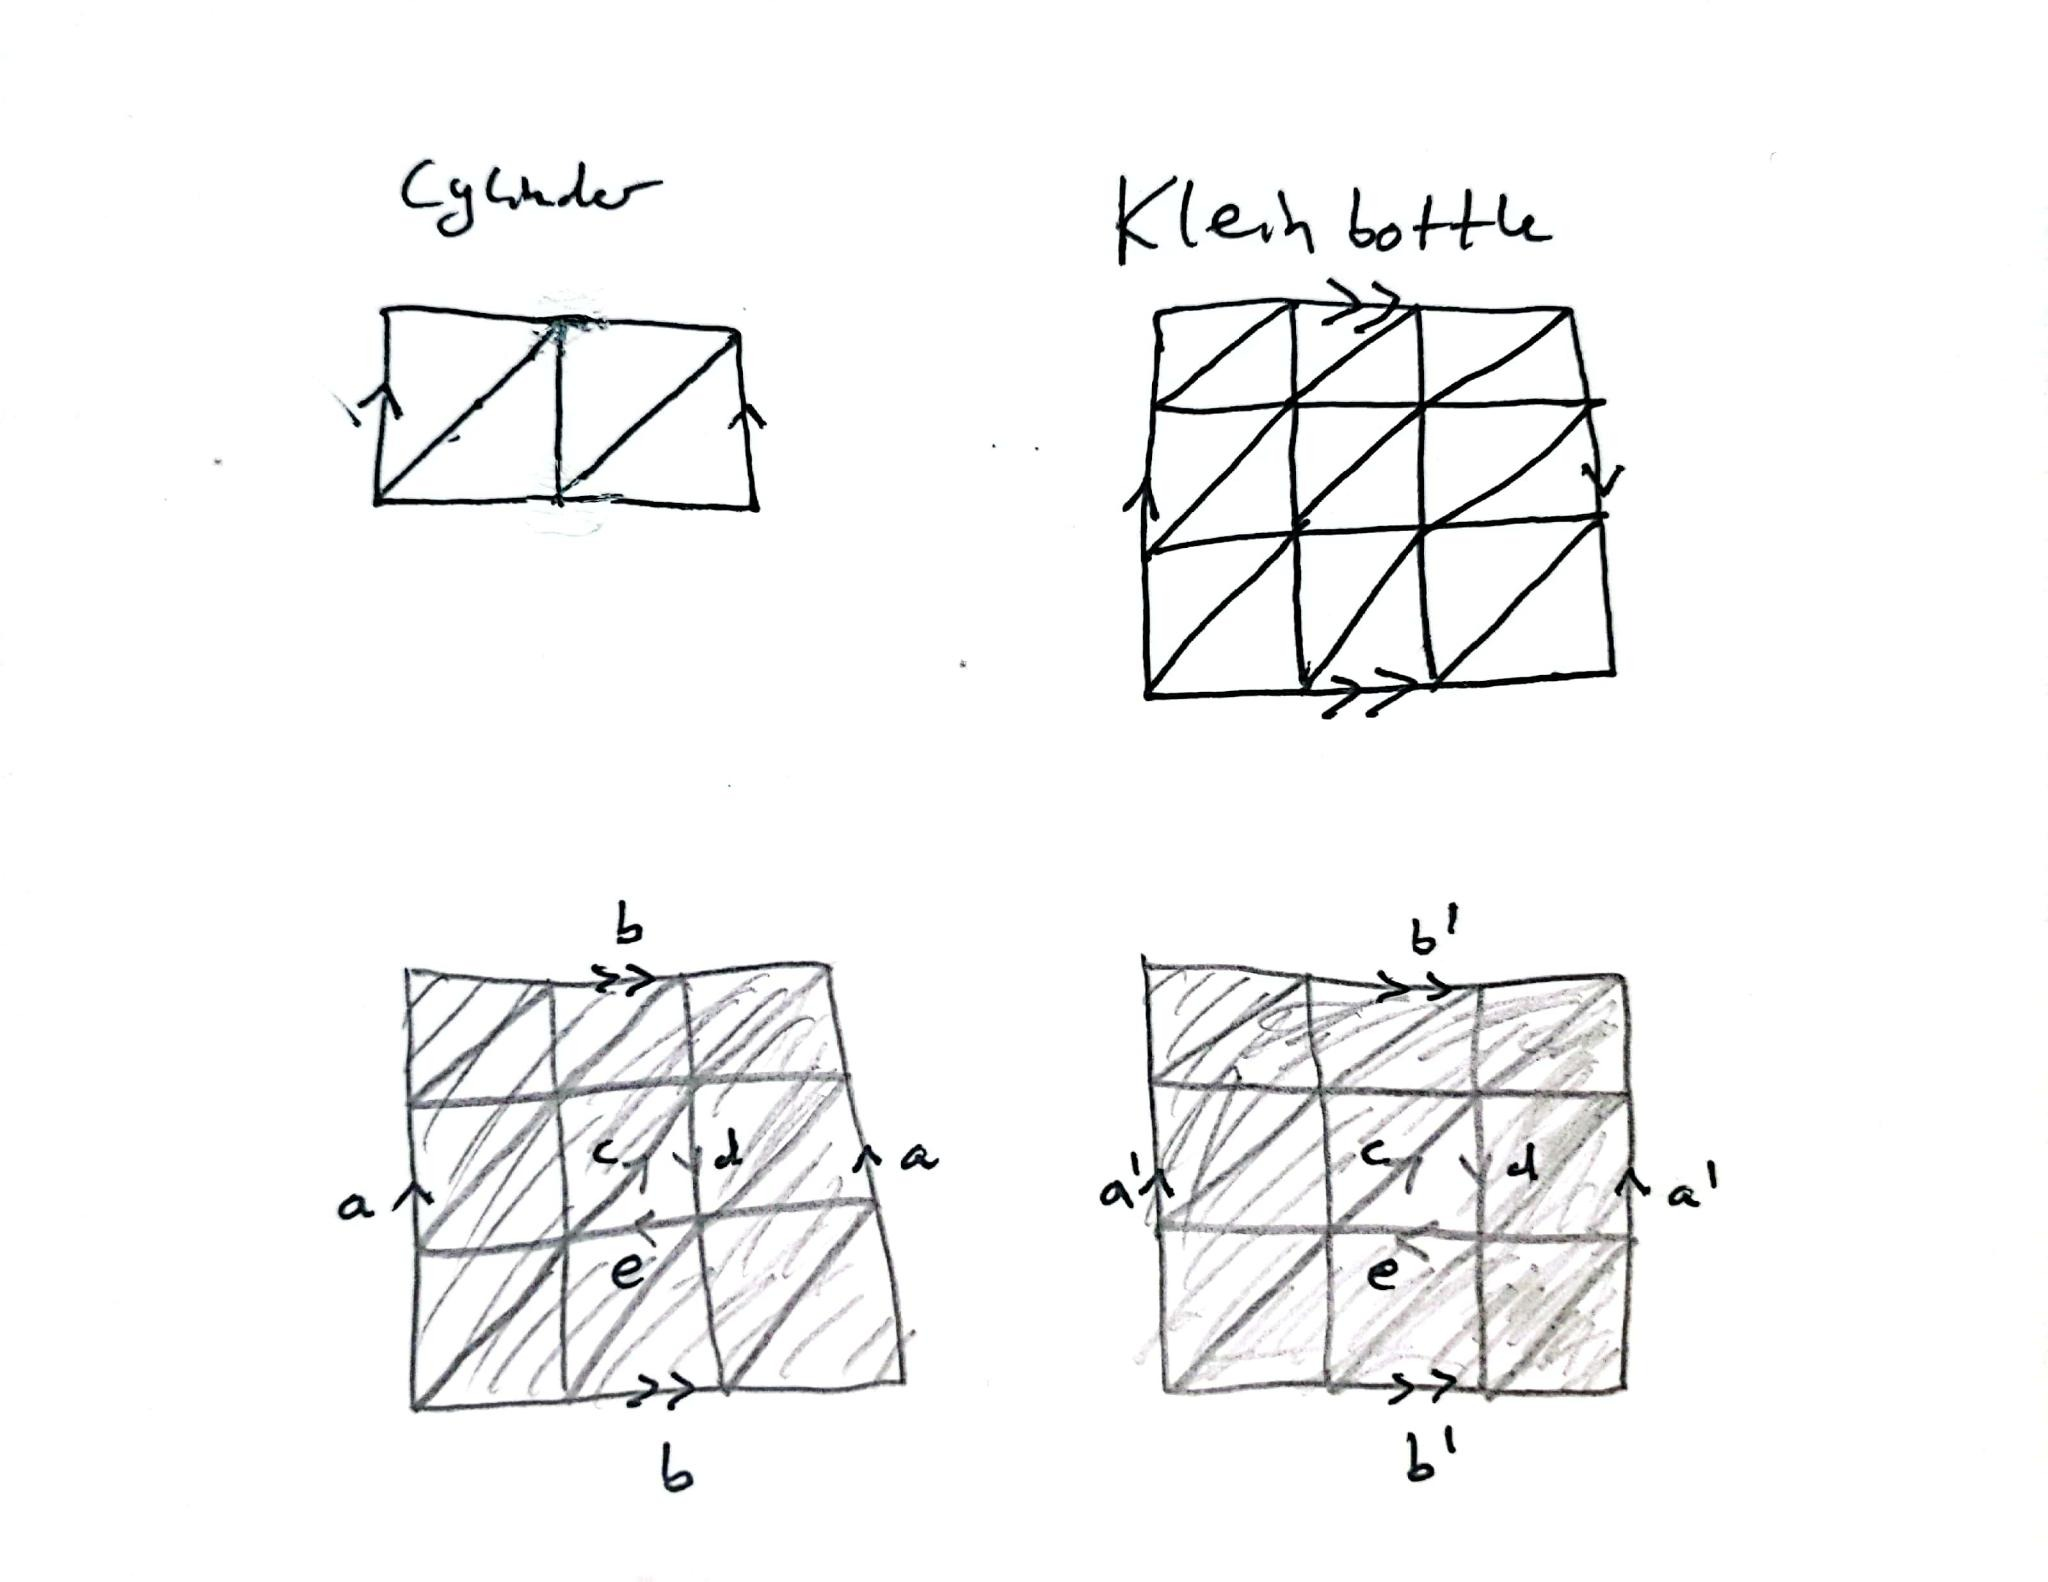
\includegraphics[width=0.8\textwidth]{1.jpeg}
        \label{fig:1-jpeg}
    \end{figure}

    Here we subdivide each square further to make sure that the
    faces are indeed simplexes as well. The cylinder thus ends up
    having a complex consisting of $4$ $2$-simplexes,
    8 $1$-simplexes and 4 $0$-simplexes.\\
    A similar decomposition can be done for the Klein bottle.\\
    For the double torus, we note that each
    square is homeomorphic to the identification space for the punctured torus,
    and we then identify the borders of the holes by gluing $c$ to $c$,
    $d$ to $d$ and $e$ to $e$ as indicated, giving a double holed torus.\\
    \linebreak
    \textbf{p. 131}\\
    \textbf{18:} Use the simplicial approximation theorem to show that the set
    of homotopy classes of maps from one polyhedron to another is always
    countable.\\
    \linebreak
    \textit{Solution:} Suppose $\left| K \right| \subset 
    \mathbb{E}^{n}$ and $\left| L \right| 
    \subset \mathbb{E}^{m}$ are polyhedra.\\
    Suppose $s  \colon \left| K^{i}\right| 
    \to \left| L \right| $ is a simplicial map. Then
    there is a finite set of vertices in $K^{i}$. Each of these vertices is
    mapped to a vertex in $L$ which also has a finite number of vertices
    - since simplicial maps take simplexes to simplexes linearly.
    Because of linearity, the simplicial map $s$ is completely determined once
    we know its effect on the vertices by extending linearly across simplexes.
    Thus there is a finite number of simplicial maps
    $\left| K^{i} \right| \to \left| L \right| $ for all $i \in
    \mathbb{N}_0$.\\
    Thus the set 
    \[
    S := \bigcup_{i \in \mathbb{N}_0} \left\{ s  \colon
    \left| K^{i} \right| \to 
\left| L \right|   \colon  \text{ is a simplicialy map} \right\} 
    \] 
    is countable. Now, for any map
    $f  \colon \left| K \right| \to \left| L \right| $, there exists an
    $m \in \mathbb{N}_0$ such that there exists a simplicial approximation
    $s  \colon \left| K^{m} \right| \to \left| L \right| $ to
    $f  \colon \left| K^{m} \right| \to \left| L \right| $. Furthermore, as
    noted on page 128, $f$ and $s$ are homotopic. But $s$ is in the
    set $S$ which is countable, so $f$ we have shown that for an arbitrary
    $f  \colon \left| K \right| \to \left| L \right| $, there exists an
    $s \in S$ such that $f$ and $s$ are in the same homotopy class.
    Thus the cardinality of the set of homotopy classes of maps is
    precisely the cardinality of $S$ which is countable.
    

















\end{document}
